\documentclass{article}\usepackage[]{graphicx}\usepackage[]{xcolor}
% maxwidth is the original width if it is less than linewidth
% otherwise use linewidth (to make sure the graphics do not exceed the margin)
\makeatletter
\def\maxwidth{ %
  \ifdim\Gin@nat@width>\linewidth
    \linewidth
  \else
    \Gin@nat@width
  \fi
}
\makeatother

\definecolor{fgcolor}{rgb}{0.345, 0.345, 0.345}
\newcommand{\hlnum}[1]{\textcolor[rgb]{0.686,0.059,0.569}{#1}}%
\newcommand{\hlstr}[1]{\textcolor[rgb]{0.192,0.494,0.8}{#1}}%
\newcommand{\hlcom}[1]{\textcolor[rgb]{0.678,0.584,0.686}{\textit{#1}}}%
\newcommand{\hlopt}[1]{\textcolor[rgb]{0,0,0}{#1}}%
\newcommand{\hlstd}[1]{\textcolor[rgb]{0.345,0.345,0.345}{#1}}%
\newcommand{\hlkwa}[1]{\textcolor[rgb]{0.161,0.373,0.58}{\textbf{#1}}}%
\newcommand{\hlkwb}[1]{\textcolor[rgb]{0.69,0.353,0.396}{#1}}%
\newcommand{\hlkwc}[1]{\textcolor[rgb]{0.333,0.667,0.333}{#1}}%
\newcommand{\hlkwd}[1]{\textcolor[rgb]{0.737,0.353,0.396}{\textbf{#1}}}%
\let\hlipl\hlkwb

\usepackage{framed}
\makeatletter
\newenvironment{kframe}{%
 \def\at@end@of@kframe{}%
 \ifinner\ifhmode%
  \def\at@end@of@kframe{\end{minipage}}%
  \begin{minipage}{\columnwidth}%
 \fi\fi%
 \def\FrameCommand##1{\hskip\@totalleftmargin \hskip-\fboxsep
 \colorbox{shadecolor}{##1}\hskip-\fboxsep
     % There is no \\@totalrightmargin, so:
     \hskip-\linewidth \hskip-\@totalleftmargin \hskip\columnwidth}%
 \MakeFramed {\advance\hsize-\width
   \@totalleftmargin\z@ \linewidth\hsize
   \@setminipage}}%
 {\par\unskip\endMakeFramed%
 \at@end@of@kframe}
\makeatother

\definecolor{shadecolor}{rgb}{.97, .97, .97}
\definecolor{messagecolor}{rgb}{0, 0, 0}
\definecolor{warningcolor}{rgb}{1, 0, 1}
\definecolor{errorcolor}{rgb}{1, 0, 0}
\newenvironment{knitrout}{}{} % an empty environment to be redefined in TeX

\usepackage{alltt}
\usepackage[brazil]{babel}
\usepackage{kpfonts}
\usepackage{indentfirst}
\usepackage{graphicx}
\usepackage{float}
\graphicspath{ {img/} }
\usepackage{amsmath}
\usepackage{array}
\usepackage{parskip}
\usepackage{csquotes}
\usepackage{siunitx}

\sisetup{
round-mode = places,
round-precision = 2,
output-decimal-marker={,},
group-separator ={.},
group-minimum-digits = 2
}


\newenvironment{conditions}
  {\par\vspace{\abovedisplayskip}\noindent\begin{tabular}{>{$}l<{$} @{${}={}$} l}}
  {\end{tabular}\par\vspace{\belowdisplayskip}}

\usepackage{multirow}


\title{Nível de Renda e Poupança}
\author{FIA Business School}
\IfFileExists{upquote.sty}{\usepackage{upquote}}{}
\begin{document}
\maketitle
\section*{Introdução}

A análise da renda auferida dentro de uma economia inicia-se sempre ao se considerar que a economia
não tem governo nem abertura para transações com o resto do mundo (suas transações com o resto do mundo somam zero).\par

Trabalha-se, inicialmente, numa \textbf{economia fechada e sem governo}, na qual prevalecem dois agentes
econômicos---trabalhadores e empresários---e a respectiva remuneração de seus fatores de produção:
mão de obra referentemente aos primeiros (trabalhadores) e bens e serviços finais no que tange aos empresários.
O desenho desse esquema está no \textit{fluxo circular de renda}.\par

\section*{Fluxo Circular de Renda}

Pelo fluxo circular de renda, temos uma das principais identidades contábeis básicas em Economia.
Quando dizemos que, contabilmente, \( A \equiv B \) não implica relação alguma de causa e efeito entre \( A \) e \( B \).\par

\begin{figure}[H]
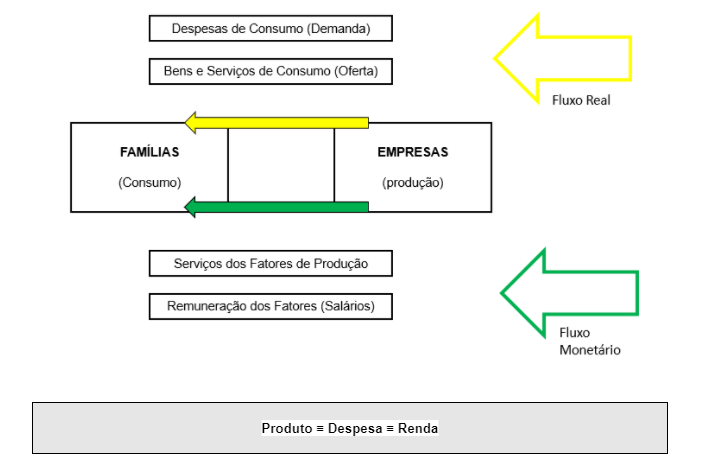
\includegraphics[width=12cm]{fluxo-circular}
\centering
\label{fluxo-circular}
\caption{Fluxo circular de renda.}
\end{figure}

Observa-se no fluxo circular de renda, numa economia fechada e sem governo, que as famílias detêm os meios de produção
(Serviço dos Fatores de Produção), representados pela mão de obra. Com a contratação e respectiva remuneração (Salários)
dessa mão de obra, as empresas geram o produto da economia -- trata-se do chamado \textbf{Fluxo Monetário} (dinheiro).
Esse produto (Bens e Serviços de Consumo) será adquirido pelos trabalhadores (famílias) que pagarão por esses bens e
serviços com os salários recebidos (Despesa de Consumo) -- trata-se do \textbf{Fluxo Real} (produtos e serviços).
Daí o nome \textit{fluxo circular}.\par

Dessa forma, a \textbf{demanda agregada} é equivalente ao \textbf{consumo da economia}.
Isso significa dizer que a procura por parte das famílias (que é a demanda agregada)
pelo produto gerado pelas empresas (que é o produto para consumo) gera a \textbf{renda da economia}.
De que forma isso ocorre? A geração de renda dá-se pela remuneração da mão de obra (salários)
por parte das empresas. Do lado das famílias, essas adquirem os bens e serviços
gerados pelas empresas e as remuneram pelos bens e serviços (pagamento do produto final).\par

Ao montarmos o fluxo circular de renda, damos o primeiro grande passo para a mensuração das \textbf{contas nacionais}.
Isso porque o produto é a principal variável macroeconômica de análise de uma economia. É por meio da geração do produto
que há a geração de renda e, portanto, todo o movimento transacional da nação.\par

Obviamente, o fluxo circular de renda é uma demonstração muito simples das relações entre agentes econômicos.
Por isso, ele considera uma economia fechada e sem governo. Ele serve para introduzir o conceito de identidades macroeconômicas,
mostrando a principal relação entre despesa e produto. As contas nacionais trabalham, como é pertinente ao mundo atual,
com economias abertas e com a presença de governos.\par

\section*{Rendas, Investimentos e Poupança}

A \textbf{Contabilidade Nacional} de um país é a mensuração dos agregados macroeconômicos dele e tem por objetivo
medir todas as transações econômicas desse país, tanto internas quanto externas, em relação ao resto do mundo.\par

As \textbf{Contas Nacionais} representam a contabilidade de um país como se este fosse um ente pessoa física ou jurídica,
prestando contas à sociedade. A análise das contas representa o passo inicial para a formulação das políticas
econômicas de uma nação.

Os principais conceitos apresentados nas Contas Nacionais são:

\begin{itemize}

  \item \textbf{Produto}: valor total dos bens e serviços produzidos numa economia num determinado período de tempo;

  \item \textbf{Renda}: a remuneração total dos fatores de produção da economia;

  \item \textbf{Consumo}: gastos realizados para atender às necessidades dos agentes econômicos;

  \item \textbf{Investimentos}: bens que ampliam a capacidade produtiva de uma nação, comumente chamados,
        em contabilidade nacional, \textit{Formação Bruta de Capital Fixo} (\(FBKF\));

  \item \textbf{Poupança}: a renda não consumida, dada pela soma da poupança do setor privado + poupança do governo +
        poupança do setor externo;

  \item \textbf{Resto do Mundo}: transações com não residentes.

\end{itemize}

Para se chegar aos valores numéricos das variáveis descritas acima, isto é, para se quantificarem essas,
a Contabilidade Nacional faz uso, primordialmente, de um método contábil com cinco contas de agregação:

\begin{itemize}
  \item \textbf{Produto Interno Bruto} (Conta de Produção): também denominado \textit{Conta-Empresas},
        na qual será apresentada a geração do produto da economia;

  \item \textbf{Renda Nacional Disponível Bruta} (Conta de Apropriação): nela será apresentado o destino dado
        à renda transacionada nesta economia. Também chamada de \textit{Conta-Famílias};

  \item \textbf{Conta de Capital}: nessa conta será apresentado o financiamento para a formação (ou não) de capital na economia;

  \item \textbf{Contas Correntes das Administrações Públicas} (Conta-Governo): nessa conta serão segregados os rendimentos
        do setor público e sua participação na economia;

  \item \textbf{Transações Correntes com o Resto do Mundo} (Conta Resto do Mundo): nela serão apresentadas as transações entre
        residentes e não residentes de uma nação. Em geral, esta é uma \enquote{conta de fechamento} da contabilidade nacional,
        como será mostrado a seguir. É também denominada \textit{Conta Setor Externo}.
\end{itemize}

Para a agregação dessas 5 contas, o sistema de contas nacionais funciona como a contabilidade de uma empresa qualquer.
Isto é, funciona como se fosse uma grande apresentação de balanço de uma empresa, no final de um dado período de tempo
(em geral, 1 ano) e  mostra-se na forma de \textbf{partidas dobradas}. Isso equivale a dizer que, nesse sistema,
\enquote{a cada débito lançado, corresponde um crédito efetuado}. Dessa forma, o sistema trabalha com equilíbrio interno das contas
(os balancetes têm de se zerar em débito e crédito) e com equilíbrio externo das contas –- o sistema tem de se zerar
como um todo, quando analisadas as 5 contas conjuntamente.

Na análise da destinação da renda auferida pelos agentes econômicos dentro de uma economia por identidade, temos, então, que:

\begin{equation}\label{eq1}
\text{Renda Agregada} = \text{Produto Agregado} = \text{Despesa Agregada}
\end{equation}

Ao supormos que as famílias não consomem toda a renda auferida, temos uma outra forma de definição da Renda:
\textbf{consumo mais poupança}.\par

Numa economia na qual as transações com o resto do mundo somam zero e as receitas do governo menos os gastos do governo
também somam zero, temos que:


\begin{equation}\label{eq2}
\begin{split}
    Y   &=    C + S
\end{split}
\end{equation}

\begin{equation}\label{eq3}
\begin{split}
    DA  &=    C + I
\end{split}
\end{equation}

onde:

\begin{conditions}
Y   &   Renda Agregada\\
C   &   Consumo\\
S   &   Poupança\\
DA  &   Despesa Agregada\\
I   &   Investimentos
\end{conditions}

Pela identidade macroeconômica básica, temos que \(Y = DA\), então:

\begin{equation}\label{eq4}
\begin{split}
C + S &= C + I
\end{split}
\end{equation}

Anulando o Consumo nos dois lados da equação:

\begin{equation}\label{eq5}
\begin{split}
S &= I
\end{split}
\end{equation}

Essa igualdade é uma das identidades mais importantes das contas nacionais.\par

\textbf{Renda Pessoal} (\(R_p\)): é a parcela da Renda Nacional recebida pelos proprietários dos fatores de produção.
Corresponde à Renda Nacional mais as Transferências, deduzidos os pagamentos ao governo que incidem sobre as
diversas formas de recebimento de renda.

\begin{equation}\label{eq6}
\begin{split}
    R_p   &=    R_n + T_g - (R_g + I_{pj} + L_r)
\end{split}
\end{equation}

onde:

\begin{conditions}
R_n   &   Renda Nacional\\
T_g   &   Transferências do Governo\\
R_g   &   Outras Receitas do Governo\\
I_{pj}&   Imposto de Renda Pago por Pessoas Jurídicas\\
L_r   &   Lucros Retidos pelas Empresas
\end{conditions}

Finalmente, temos o conceito de:\par

\textbf{Renda Pessoal disponível} (\(R_{pd}\)): é o valor da renda nacional que as pessoas podem gastar.
Ela é formada pelos salários, renda da previdência social, aluguéis, dividendos e juros,
exclusos os impostos diretos (cobrados sobre a renda gerada) que as pessoas têm de pagar.


\begin{equation}\label{eq7}
\begin{split}
    R_{pd}   &=    R_p - I_d
\end{split}
\end{equation}

onde:

\begin{conditions}
I_d   &   Impostos Diretos
\end{conditions}


\section*{Nível de Emprego}

O nível de emprego mede a proporção da \textbf{População Economicamente Ativa} (\(PEA\)) de um país que está empregada.
Entende-se \(PEA\) ou força de trabalho como o conjunto de indivíduos em idade ativa e capacitados ao trabalho
que estão empregados (\(E\)) ou desempregados que buscam emprego (\(D\)), portanto (\(PEA = E + D\)).\par

Quando uma economia cresce, o nível de emprego sobe, já que aumentam as oportunidades de trabalho, seja pelo
surgimento de novas ocupações, seja pela ampliação do número de vagas em ocupações já existentes.
Quando há uma contração da atividade econômica ou uma recessão, o nível de emprego cai. As variações no emprego
acompanham, portanto, os ciclos econômicos registrados nos países.\par

Existe também a relação inversa. Políticas de estímulo à criação de emprego são poderosas para impulsionar o
crescimento do \(PIB\), especialmente em épocas de crise econômica ou recessão.\par

Normalmente, quando nos referimos ao nível de emprego usamos a \textbf{taxa de desemprego} como indicador.
Ela mede a incapacidade do sistema econômico em prover ocupação remunerada para todos os que a desejam.
A taxa de desemprego contabiliza os indivíduos que fazem parte da \(PEA\) e não encontram trabalho remunerado.
Estatisticamente, a taxa de desemprego é igual ao número de desempregados (\(D\)) dividido pelo total da \(PEA\), ou seja:


\begin{equation}\label{eq8}
\begin{split}
\text{Taxa de Desemprego} &= \frac{D}{PEA}\\
                          &= \frac{D}{E + D}
\end{split}
\end{equation}

A \textbf{taxa de desemprego} ou o \textbf{nível de emprego} são indicadores muito importantes do bem-estar de uma sociedade.

\section*{Nível de Salários}

O \textbf{nível salarial} de uma economia também é um indicador social. Ele reflete o estado do mercado de trabalho
e da própria economia. Quando existe expansão econômica, pode haver um desequilíbrio entre oferta e demanda
de trabalhadores, fato que normalmente leva a um aumento dos salários pagos. Além disso, em períodos de
crescimento, os trabalhadores têm maiores chances de mobilidade em direção a empregos de maior remuneração
e mesmo de promoção. O nível de salário também é influenciado pela \textbf{política salarial} vigente.\par

É importante, porém, distinguir \textbf{salário nominal} de \textbf{salário real}.
A diferença entre o salário nominal e real é a \textbf{inflação}. Enquanto a evolução do salário nominal é condicionada
pela política salarial e ocorrência de desemprego, a evolução do salário real é determinada pelo ritmo de
crescimento dos preços. Caso a inflação seja elevada, os ganhos de salário nominal podem ser anulados.\par

O nível de salário real também está atrelado à \textbf{produtividade do trabalho}. Se a produtividade crescer, ela
poderá ser incorporada ao salário real para manter (inalterada) a distribuição da renda entre salários e lucros.

\begin{equation}\label{eq9}
\begin{split}
    W_r   &=    \frac{w}{IP}
\end{split}
\end{equation}

onde:

\begin{conditions}
W_r   &   Salário real\\
w     &   Salário nominal\\
IP    &   Índice de preços (inflação)\\
\end{conditions}

\section*{Arrecadação e Gastos do Governo}

O governo aparece nas contas nacionais como provedor de bens públicos, isto é, aqueles que não
seriam supridos pelo mercado, como saneamento básico, construção de estradas, portos, segurança, etc.
Para prover tais bens à nação, o governo dispõe da arrecadação de impostos e essa é a sua fonte de
receitas. Os impostos arrecadados são classificados em:\par

\textbf{mpostos Diretos}: são cobrados sobre a renda gerada que as pessoas (físicas ou jurídicas) têm a pagar,
por exemplo: o Imposto de Renda (IR) e o Imposto sobre Propriedade Territorial Urbana (IPTU);\par

\textbf{Impostos Indiretos}: são cobrados do consumidor final (pessoa física ou jurídica), como o Imposto sobre
Circulação de Mercadorias e Serviços (ICMS) e o Imposto sobre Produtos Industrializados (IPI).\par

Ao incluirmos o governo na economia, passamos a trabalhar com uma economia fechada (na qual as transações
com o resto do mundo somam zero) e com o governo. A identidade básica da renda dessa economia passa a ser
representada pela seguinte equação:

\begin{equation}\label{eq10}
\begin{split}
    Y   &=    C + S + T
\end{split}
\end{equation}

onde:

\begin{conditions}
Y   &   Renda\\
C   &   Consumo\\
S   &   Poupança\\
T   &   Impostos Totais
\end{conditions}

Considerando-se os gastos públicos (gastos do governo), reescrevemos também a despesa agregada:

\begin{equation}\label{eq11}
\begin{split}
    DA   &=    C + I + G
\end{split}
\end{equation}

Novamente, pela identidade macroeconômica básica (\(Y = DA\)) e com as transações com o resto do mundo
somando zero (economia fechada), temos que:

\begin{equation}\label{eq12}
\begin{split}
    C + S + T   &=    C + I + G
\end{split}
\end{equation}

Anulando o Consumo nos dois lados da equação:

\begin{equation}\label{eq13}
\begin{split}
    S – I   &=    T - G
\end{split}
\end{equation}

A interpretação dessa segunda identidade mostra-nos a necessidade da geração de poupança pelo governo,
isto é, que o governo arrecade mais do que gaste (\(T > G\)) ou, no mínimo, mantenha seu orçamento equilibrado
(\(T = G\)) para que não precise ser financiado pelo setor privado.\par

Na presença de déficit no setor público (\(T < G\)), a economia deve gerar um excesso de poupança no setor privado
(\(S > I\)) para financiar o governo, preterindo os investimentos em \(FBKF\) (formação bruta de capital fixo).

\section*{Transações com o Setor Externo}

Ao incluirmos o \textbf{resto do mundo} (termo comumente utilizado em economia para descrever as transações feitas
com não residentes, isto é, agentes econômicos locados em outros países) passamos a analisar uma economia
aberta ao livre fluxo de capitais, conforme as identidades macroeconômicas apresentadas abaixo:

\begin{equation}\label{eq14}
\begin{split}
    DA    &=    C + I + G + (X – M)
\end{split}
\end{equation}

onde:

\begin{conditions}
X – M   &   Gastos líquidos do setor externo ou exportações líquidas
\end{conditions}

Rearranjado a equação e considerando que \(Y = DA\), temos que:

\begin{equation}\label{eq15}
\begin{split}
    (Y + M) &= C + I + G + X
\end{split}
\end{equation}

onde:

\begin{conditions}
Y   &   Renda\\
M   &   Importações\\
C   &   Consumo\\
I   &   Investimentos\\
G   &   Consumo ou gastos do governo\\
X   &   Exportações\\
\end{conditions}

Do lado esquerdo da equação, temos agora a oferta agregada da economia (\(Y + M\)).\par

Do lado direito da equação, temos a demanda agregada da economia (\(C + I + G + X\)).\par

Teremos, então, as identidades que se seguem:\par

Ao considerarmos \textbf{a ótica da utilização de renda auferida na economia}:

\begin{equation}\label{eq16}
\begin{split}
    Y &= C + S + T + M
\end{split}
\end{equation}

Isso nos diz que os agentes econômicos, numa economia aberta, empregam sua renda em consumo,
poupança, impostos e importações.\par

Ao considerarmos \textbf{a ótica da despesa agregada}:


\begin{equation}\label{eq17}
\begin{split}
    Y &= C + I + G + X
\end{split}
\end{equation}

Chegamos, então, à terceira identidade básica em macroeconomia:

\begin{equation}\label{eq18}
\begin{split}
    C + S + T + M &= C + I + G + X
\end{split}
\end{equation}

Anulando o Consumo nos dois lados e rearranjando a equação:

\begin{equation}\label{eq19}
\begin{split}
    (X - M) &= (S - I) + (T - G)
\end{split}
\end{equation}

Observamos que, na presença de déficit no setor externo (\(X < M\)), há déficit no
setor privado (\(S – I\)) ou nas contas do governo (\(T – G\)), ou em ambos os setores da economia.

\section*{Conta de Produção (Produto Interno Bruto)}

A primeira grande agregação contábil em Contas Nacionais é a \textbf{Conta de Produção} (PIB),
que traz a geração da \textbf{Oferta Global} e da \textbf{Demanda Global} da economia de uma nação.


\begin{table}[H]
\centering
\begin{tabular}{ |p{7cm}|p{4cm}|  }
 \hline
 \multicolumn{2}{|c|}{Conta de Produção (PIB)}\\
 \hline
 \textbf{DÉBITO}                                  &   \textbf{CRÉDITO}\\
 \hline
 \textbf{Produto Interno Bruto a custo de fatores}&   (+) Consumo das familías\\
 \hline
 (+) Salários                                     &   \\
 \hline
 \textbf{Excedente Operacional Bruto}             &   (+) Consumo do governo\\
 \hline
 (+) Juros                                        &   \\
 \hline
 (+) Lucros                                       &   (+) \(IBK\) ou \(IBKF\)\\
 \hline
 (+) Aluguéis                                     &   (+) Variação de Estoques\\
 \hline
 (+) Dividendos                                   &   \\
 \hline
 = \textbf{Renda Interna Bruta a custo de fatores}&   \textbf{Exportações Líquidas}\\
 \hline
 (+) Tributos Indiretos                           &   (+) Exportações\\
 \hline
 (-) Subsídios                                    &   (-) Importações\\
 \hline
  = \(\mathbf{PIB_{pm}}\)                         &   = \(\mathbf{DIB_{pm}}\)\\
 \hline
\end{tabular}
\end{table}

onde:

\begin{conditions}
IBK       &   Investimentos em Ativos Fixos\\
IBKF      &   Formação Bruta de Capital Fixo\\
PIB_{pm}  &   Produto Interno Bruto a preço de mercado\\
DIB_{pm}  &   Dispêndio Interno Bruto a preço de mercado\\
\end{conditions}


Na conta de produção (PIB), lança-se a crédito o pagamento às empresas pelos bens e serviços finais 
produzidos por elas, quer para consumo doméstico das famílias e do governo, quer para consumo externo, 
por meio de exportações.\par

Lançam-se, também, a crédito das empresas, seus investimentos em Formação Bruta de Capital Fixo (FBKF) e estoques. 
A FBKF representa o investimento da empresa nela mesma e na economia como um todo, isto é, em capacidade produtiva, 
por meio de seu parque produtivo, representado pelas máquinas e equipamentos.\par

A variação de estoques dará, em boa medida, a necessidade ou não de ampliação dos investimentos das empresas e, 
por isso, representa uma importante variável para políticas industriais (numa forma mais restrita, de análise 
microeconômica de análise conjuntural) e para políticas econômicas (numa forma macroeconômica de análise conjuntural). 
\textbf{Dessa forma, os lançamentos a crédito da conta produção resultam na procura total de uma economia}.\par

Com a remuneração dos seus bens e serviços, as empresas conseguem remunerar os fatores de produção da
economia, que serão, então, lançados a débito na conta de produção. Os principais fatores são: salários,
juros, lucros e aluguéis. Contudo, ao considerarmos uma economia aberta, é necessária a contabilização
das importações e da Renda Líquida Transacionada com o Exterior, que representam a remuneração dos
fatores externos de produção e dos não residentes no país.\par

E, ao considerarmos o governo, temos a "remuneração" do ente público, por meio da arrecadação líquida 
(arrecadação descontada de transferências e subsídios governamentais à economia). Dessa forma, os lançamentos 
a débito da conta produção resultam na oferta total de uma economia, pela remuneração dos seus fatores de produção.\par

\section*{Produto Interno Bruto}

O \textbf{Produto Interno Bruto} (PIB) é um importante indicador econômico que representa (em valores monetários \$\$\$) 
a soma de todos os bens e serviços finais realizados (produzidos) durante um determinado período (geralmente um ano) 
numa determinada região (geralmente um país).\par

O termo \enquote{bens e serviços finais} é empregado para ilustrar o que é contabilizado na soma do PIB 
(somente o que é produzido no final de uma cadeia produtiva). Dessa forma, evita-se a \enquote{dupla contagem} 
ocasionada com bens e serviços de consumo intermediários. Exemplo: o valor de uma moto produzida por uma empresa 
é contabilizada na soma do PIB pelo último elo da cadeia, ou seja, descontando o valor da produção das peças realizadas 
por outras empresas para a montagem final da moto. Se fosse somado no PIB o valor de cada peça produzida na cadeia 
produtiva poder-se-ia chegar ao dobro do valor que deveria ser.\par

Sabemos o que representa o PIB, mas como é calculado na prática? Os dois principais modelos para se chegar ao mesmo 
número (valor do PIB) são:\par

\textbf{Óptica da Produção}. É justamente a soma do valor agregado em cada fase de produção exemplificada anteriormente. 
Na prática é muito complicado o seu cálculo, pois nem todas as empresas são obrigadas a informar publicamente suas 
demonstrações financeiras, o que torna o cálculo falho. Além disso, devem ser considerados todos os fatores de produção 
entre os setores primário (matéria-prima), secundário (transformação) e terciário (serviços). 
Portanto é praticamente impossível, pela falta de informação, saber o relacionamento das diversas cadeias produtivas, 
envolvendo todos os setores da economia, para se chegar ao correto valor adicionado que será utilizado no cálculo final 
do PIB. Veja um exemplo matemático:\par 


\begin{table}[H]
\centering
\resizebox{\textwidth}{!}{%
\begin{tabular}{ |p{3cm}|p{3cm}|p{3cm}|p{3cm}|  }
 \hline
 \multicolumn{4}{|c|}{Cálculo do PIB (Óptica da Produção)}\\
 \hline 
 \textbf{Exemplo de cadeia produtiva}            &
 \textbf{Produto do setor}                       &
 \textbf{Compras entre a cadeia produtiva}       &
 \textbf{Valor adicionado em cada fase}          \\
 \hline
 Agricultor vende para Indústria        & R\$\num{1000}           &   ---             &   R\$\num{1000}   \\
 \hline
 Indústria vende para Varejista         & R\$\num{3000}           &   R\$\num{1000}   &   R\$\num{2000}   \\
 \hline
 Varejista vende para Consumidor Final  & R\$\num{7000}           &   R\$\num{3000}   &   R\$\num{4000}   \\
 \hline
 \textbf{Produto Interno}               & \textbf{R\$\num{7000}}  &   ---             &   ---             \\
 \hline
\end{tabular}}
\end{table}

\textbf{Óptica do Dispêndio}. É o \enquote{jeitinho} que foi dado para solucionar o problema de 
falta de informação do valor adicionado em cada fase das cadeias produtivas. O método de cálculo 
pela óptica do dispêndio é mais simples, pois no mercado formal existem as notas fiscais de consumo.\par

Para o cálculo leva-se em consideração a soma do consumo das Famílias (pessoas), Empresas, Governo e 
a diferença do que é consumido por estrangeiros menos o que é consumido de importação.\par

\begin{table}[H]
\centering
\resizebox{\textwidth}{!}{%
\begin{tabular}{ |p{2cm}|p{2cm}|p{2cm}|p{2cm}|p{2cm}|  }
 \hline
 \multicolumn{5}{|c|}{Cálculo do PIB (Óptica do Dispêndio)}\\
 \hline 
 \textbf{PIB =} &
 \textbf{C +}   &
 \textbf{I +}   &
 \textbf{G +}   &
 \textbf{(E - I)}\\
 \hline
 \multicolumn{1}{|l|}{Produto Interno Bruto}  &
 \multicolumn{1}{l|}{Consumo das Famílias} &
 \multicolumn{1}{l|}{Investimentos}  &
 \multicolumn{1}{l|}{Gastos do Governo}  &
 \multicolumn{1}{l|}{Exportação - Importação}\\
 \hline
\end{tabular}}
\end{table}

Por ser uma das fórmulas mais importantes da economia, alguns autores utilizam a apresentação 
dela em inglês, inclusive isso já ocorreu em exames passados, portanto apresentamos notação 
matemática na língua inglesa. Repare que é muito similar à notação na língua portuguesa.\par

\begin{table}[H]
\centering
\resizebox{\textwidth}{!}{%
\begin{tabular}{ |p{2cm}|p{2cm}|p{2cm}|p{2cm}|p{2cm}|  }
 \hline
 \multicolumn{5}{|c|}{Cálculo do PIB (Óptica do Dispêndio)}\\
 \hline 
 \textbf{GPD =} &
 \textbf{C +}   &
 \textbf{I +}   &
 \textbf{G +}   &
 \textbf{(NX)}\\
 \hline
 \multicolumn{1}{|l|}{\textbf{G}ross \textbf{D}omestic \textbf{P}roduct}  &
 \multicolumn{1}{l|}{\textbf{P}rivate \textbf{C}onsumption} &
 \multicolumn{1}{l|}{\textbf{G}ross \textbf{I}nvestment}  &
 \multicolumn{1}{l|}{\textbf{G}overnment \textbf{S}pending}  &
 \multicolumn{1}{l|}{\textbf{N}et E\textbf{x}ports}\\
 \hline
\end{tabular}}
\end{table}


















\end{document}
